\documentclass[11pt]{article}

    \usepackage[breakable]{tcolorbox}
    \usepackage{parskip} % Stop auto-indenting (to mimic markdown behaviour)
    
    \usepackage{iftex}
    \ifPDFTeX
    	\usepackage[T1]{fontenc}
    	\usepackage{mathpazo}
    \else
    	\usepackage{fontspec}
    \fi

    \usepackage{graphicx} %package to manage images
    \graphicspath{ {./images/} }
    \usepackage{wrapfig}
    
    % Basic figure setup, for now with no caption control since it's done
    % automatically by Pandoc (which extracts ![](path) syntax from Markdown).
    \usepackage{graphicx}
    % Maintain compatibility with old templates. Remove in nbconvert 6.0
    \let\Oldincludegraphics\includegraphics
    % Ensure that by default, figures have no caption (until we provide a
    % proper Figure object with a Caption API and a way to capture that
    % in the conversion process - todo).
    \usepackage{caption}
    \DeclareCaptionFormat{nocaption}{}
    \captionsetup{format=nocaption,aboveskip=0pt,belowskip=0pt}

    \usepackage[Export]{adjustbox} % Used to constrain images to a maximum size
    \adjustboxset{max size={0.9\linewidth}{0.9\paperheight}}
    \usepackage{float}
    \floatplacement{figure}{H} % forces figures to be placed at the correct location
    \usepackage{xcolor} % Allow colors to be defined
    \usepackage{enumerate} % Needed for markdown enumerations to work
    \usepackage{geometry} % Used to adjust the document margins
    \usepackage{amsmath} % Equations
    \usepackage{amssymb} % Equations
    \usepackage{textcomp} % defines textquotesingle
    % Hack from http://tex.stackexchange.com/a/47451/13684:
    \AtBeginDocument{%
        \def\PYZsq{\textquotesingle}% Upright quotes in Pygmentized code
    }
    \usepackage{upquote} % Upright quotes for verbatim code
    \usepackage{eurosym} % defines \euro
    \usepackage[mathletters]{ucs} % Extended unicode (utf-8) support
    \usepackage{fancyvrb} % verbatim replacement that allows latex
    \usepackage{grffile} % extends the file name processing of package graphics 
                         % to support a larger range
    \makeatletter % fix for grffile with XeLaTeX
    \def\Gread@@xetex#1{%
      \IfFileExists{"\Gin@base".bb}%
      {\Gread@eps{\Gin@base.bb}}%
      {\Gread@@xetex@aux#1}%
    }
    \makeatother

    % The hyperref package gives us a pdf with properly built
    % internal navigation ('pdf bookmarks' for the table of contents,
    % internal cross-reference links, web links for URLs, etc.)
    \usepackage{hyperref}
    % The default LaTeX title has an obnoxious amount of whitespace. By default,
    % titling removes some of it. It also provides customization options.
    \usepackage{titling}
    \usepackage{longtable} % longtable support required by pandoc >1.10
    \usepackage{booktabs}  % table support for pandoc > 1.12.2
    \usepackage[inline]{enumitem} % IRkernel/repr support (it uses the enumerate* environment)
    \usepackage[normalem]{ulem} % ulem is needed to support strikethroughs (\sout)
                                % normalem makes italics be italics, not underlines
    \usepackage{mathrsfs}
    

    
    % Colors for the hyperref package
    \definecolor{urlcolor}{rgb}{0,.145,.698}
    \definecolor{linkcolor}{rgb}{.71,0.21,0.01}
    \definecolor{citecolor}{rgb}{.12,.54,.11}

    % ANSI colors
    \definecolor{ansi-black}{HTML}{3E424D}
    \definecolor{ansi-black-intense}{HTML}{282C36}
    \definecolor{ansi-red}{HTML}{E75C58}
    \definecolor{ansi-red-intense}{HTML}{B22B31}
    \definecolor{ansi-green}{HTML}{00A250}
    \definecolor{ansi-green-intense}{HTML}{007427}
    \definecolor{ansi-yellow}{HTML}{DDB62B}
    \definecolor{ansi-yellow-intense}{HTML}{B27D12}
    \definecolor{ansi-blue}{HTML}{208FFB}
    \definecolor{ansi-blue-intense}{HTML}{0065CA}
    \definecolor{ansi-magenta}{HTML}{D160C4}
    \definecolor{ansi-magenta-intense}{HTML}{A03196}
    \definecolor{ansi-cyan}{HTML}{60C6C8}
    \definecolor{ansi-cyan-intense}{HTML}{258F8F}
    \definecolor{ansi-white}{HTML}{C5C1B4}
    \definecolor{ansi-white-intense}{HTML}{A1A6B2}
    \definecolor{ansi-default-inverse-fg}{HTML}{FFFFFF}
    \definecolor{ansi-default-inverse-bg}{HTML}{000000}

    % commands and environments needed by pandoc snippets
    % extracted from the output of `pandoc -s`
    \providecommand{\tightlist}{%
      \setlength{\itemsep}{0pt}\setlength{\parskip}{0pt}}
    \DefineVerbatimEnvironment{Highlighting}{Verbatim}{commandchars=\\\{\}}
    % Add ',fontsize=\small' for more characters per line
    \newenvironment{Shaded}{}{}
    \newcommand{\KeywordTok}[1]{\textcolor[rgb]{0.00,0.44,0.13}{\textbf{{#1}}}}
    \newcommand{\DataTypeTok}[1]{\textcolor[rgb]{0.56,0.13,0.00}{{#1}}}
    \newcommand{\DecValTok}[1]{\textcolor[rgb]{0.25,0.63,0.44}{{#1}}}
    \newcommand{\BaseNTok}[1]{\textcolor[rgb]{0.25,0.63,0.44}{{#1}}}
    \newcommand{\FloatTok}[1]{\textcolor[rgb]{0.25,0.63,0.44}{{#1}}}
    \newcommand{\CharTok}[1]{\textcolor[rgb]{0.25,0.44,0.63}{{#1}}}
    \newcommand{\StringTok}[1]{\textcolor[rgb]{0.25,0.44,0.63}{{#1}}}
    \newcommand{\CommentTok}[1]{\textcolor[rgb]{0.38,0.63,0.69}{\textit{{#1}}}}
    \newcommand{\OtherTok}[1]{\textcolor[rgb]{0.00,0.44,0.13}{{#1}}}
    \newcommand{\AlertTok}[1]{\textcolor[rgb]{1.00,0.00,0.00}{\textbf{{#1}}}}
    \newcommand{\FunctionTok}[1]{\textcolor[rgb]{0.02,0.16,0.49}{{#1}}}
    \newcommand{\RegionMarkerTok}[1]{{#1}}
    \newcommand{\ErrorTok}[1]{\textcolor[rgb]{1.00,0.00,0.00}{\textbf{{#1}}}}
    \newcommand{\NormalTok}[1]{{#1}}
    
    % Additional commands for more recent versions of Pandoc
    \newcommand{\ConstantTok}[1]{\textcolor[rgb]{0.53,0.00,0.00}{{#1}}}
    \newcommand{\SpecialCharTok}[1]{\textcolor[rgb]{0.25,0.44,0.63}{{#1}}}
    \newcommand{\VerbatimStringTok}[1]{\textcolor[rgb]{0.25,0.44,0.63}{{#1}}}
    \newcommand{\SpecialStringTok}[1]{\textcolor[rgb]{0.73,0.40,0.53}{{#1}}}
    \newcommand{\ImportTok}[1]{{#1}}
    \newcommand{\DocumentationTok}[1]{\textcolor[rgb]{0.73,0.13,0.13}{\textit{{#1}}}}
    \newcommand{\AnnotationTok}[1]{\textcolor[rgb]{0.38,0.63,0.69}{\textbf{\textit{{#1}}}}}
    \newcommand{\CommentVarTok}[1]{\textcolor[rgb]{0.38,0.63,0.69}{\textbf{\textit{{#1}}}}}
    \newcommand{\VariableTok}[1]{\textcolor[rgb]{0.10,0.09,0.49}{{#1}}}
    \newcommand{\ControlFlowTok}[1]{\textcolor[rgb]{0.00,0.44,0.13}{\textbf{{#1}}}}
    \newcommand{\OperatorTok}[1]{\textcolor[rgb]{0.40,0.40,0.40}{{#1}}}
    \newcommand{\BuiltInTok}[1]{{#1}}
    \newcommand{\ExtensionTok}[1]{{#1}}
    \newcommand{\PreprocessorTok}[1]{\textcolor[rgb]{0.74,0.48,0.00}{{#1}}}
    \newcommand{\AttributeTok}[1]{\textcolor[rgb]{0.49,0.56,0.16}{{#1}}}
    \newcommand{\InformationTok}[1]{\textcolor[rgb]{0.38,0.63,0.69}{\textbf{\textit{{#1}}}}}
    \newcommand{\WarningTok}[1]{\textcolor[rgb]{0.38,0.63,0.69}{\textbf{\textit{{#1}}}}}
    
    
    % Define a nice break command that doesn't care if a line doesn't already
    % exist.
    \def\br{\hspace*{\fill} \\* }
    % Math Jax compatibility definitions
    \def\gt{>}
    \def\lt{<}
    \let\Oldtex\TeX
    \let\Oldlatex\LaTeX
    \renewcommand{\TeX}{\textrm{\Oldtex}}
    \renewcommand{\LaTeX}{\textrm{\Oldlatex}}
    % Document parameters
    % Document title
    \title{2-factor-Hull-White\_model\_calibration}
    
    
    
    
    
% Pygments definitions
\makeatletter
\def\PY@reset{\let\PY@it=\relax \let\PY@bf=\relax%
    \let\PY@ul=\relax \let\PY@tc=\relax%
    \let\PY@bc=\relax \let\PY@ff=\relax}
\def\PY@tok#1{\csname PY@tok@#1\endcsname}
\def\PY@toks#1+{\ifx\relax#1\empty\else%
    \PY@tok{#1}\expandafter\PY@toks\fi}
\def\PY@do#1{\PY@bc{\PY@tc{\PY@ul{%
    \PY@it{\PY@bf{\PY@ff{#1}}}}}}}
\def\PY#1#2{\PY@reset\PY@toks#1+\relax+\PY@do{#2}}

\expandafter\def\csname PY@tok@w\endcsname{\def\PY@tc##1{\textcolor[rgb]{0.73,0.73,0.73}{##1}}}
\expandafter\def\csname PY@tok@c\endcsname{\let\PY@it=\textit\def\PY@tc##1{\textcolor[rgb]{0.25,0.50,0.50}{##1}}}
\expandafter\def\csname PY@tok@cp\endcsname{\def\PY@tc##1{\textcolor[rgb]{0.74,0.48,0.00}{##1}}}
\expandafter\def\csname PY@tok@k\endcsname{\let\PY@bf=\textbf\def\PY@tc##1{\textcolor[rgb]{0.00,0.50,0.00}{##1}}}
\expandafter\def\csname PY@tok@kp\endcsname{\def\PY@tc##1{\textcolor[rgb]{0.00,0.50,0.00}{##1}}}
\expandafter\def\csname PY@tok@kt\endcsname{\def\PY@tc##1{\textcolor[rgb]{0.69,0.00,0.25}{##1}}}
\expandafter\def\csname PY@tok@o\endcsname{\def\PY@tc##1{\textcolor[rgb]{0.40,0.40,0.40}{##1}}}
\expandafter\def\csname PY@tok@ow\endcsname{\let\PY@bf=\textbf\def\PY@tc##1{\textcolor[rgb]{0.67,0.13,1.00}{##1}}}
\expandafter\def\csname PY@tok@nb\endcsname{\def\PY@tc##1{\textcolor[rgb]{0.00,0.50,0.00}{##1}}}
\expandafter\def\csname PY@tok@nf\endcsname{\def\PY@tc##1{\textcolor[rgb]{0.00,0.00,1.00}{##1}}}
\expandafter\def\csname PY@tok@nc\endcsname{\let\PY@bf=\textbf\def\PY@tc##1{\textcolor[rgb]{0.00,0.00,1.00}{##1}}}
\expandafter\def\csname PY@tok@nn\endcsname{\let\PY@bf=\textbf\def\PY@tc##1{\textcolor[rgb]{0.00,0.00,1.00}{##1}}}
\expandafter\def\csname PY@tok@ne\endcsname{\let\PY@bf=\textbf\def\PY@tc##1{\textcolor[rgb]{0.82,0.25,0.23}{##1}}}
\expandafter\def\csname PY@tok@nv\endcsname{\def\PY@tc##1{\textcolor[rgb]{0.10,0.09,0.49}{##1}}}
\expandafter\def\csname PY@tok@no\endcsname{\def\PY@tc##1{\textcolor[rgb]{0.53,0.00,0.00}{##1}}}
\expandafter\def\csname PY@tok@nl\endcsname{\def\PY@tc##1{\textcolor[rgb]{0.63,0.63,0.00}{##1}}}
\expandafter\def\csname PY@tok@ni\endcsname{\let\PY@bf=\textbf\def\PY@tc##1{\textcolor[rgb]{0.60,0.60,0.60}{##1}}}
\expandafter\def\csname PY@tok@na\endcsname{\def\PY@tc##1{\textcolor[rgb]{0.49,0.56,0.16}{##1}}}
\expandafter\def\csname PY@tok@nt\endcsname{\let\PY@bf=\textbf\def\PY@tc##1{\textcolor[rgb]{0.00,0.50,0.00}{##1}}}
\expandafter\def\csname PY@tok@nd\endcsname{\def\PY@tc##1{\textcolor[rgb]{0.67,0.13,1.00}{##1}}}
\expandafter\def\csname PY@tok@s\endcsname{\def\PY@tc##1{\textcolor[rgb]{0.73,0.13,0.13}{##1}}}
\expandafter\def\csname PY@tok@sd\endcsname{\let\PY@it=\textit\def\PY@tc##1{\textcolor[rgb]{0.73,0.13,0.13}{##1}}}
\expandafter\def\csname PY@tok@si\endcsname{\let\PY@bf=\textbf\def\PY@tc##1{\textcolor[rgb]{0.73,0.40,0.53}{##1}}}
\expandafter\def\csname PY@tok@se\endcsname{\let\PY@bf=\textbf\def\PY@tc##1{\textcolor[rgb]{0.73,0.40,0.13}{##1}}}
\expandafter\def\csname PY@tok@sr\endcsname{\def\PY@tc##1{\textcolor[rgb]{0.73,0.40,0.53}{##1}}}
\expandafter\def\csname PY@tok@ss\endcsname{\def\PY@tc##1{\textcolor[rgb]{0.10,0.09,0.49}{##1}}}
\expandafter\def\csname PY@tok@sx\endcsname{\def\PY@tc##1{\textcolor[rgb]{0.00,0.50,0.00}{##1}}}
\expandafter\def\csname PY@tok@m\endcsname{\def\PY@tc##1{\textcolor[rgb]{0.40,0.40,0.40}{##1}}}
\expandafter\def\csname PY@tok@gh\endcsname{\let\PY@bf=\textbf\def\PY@tc##1{\textcolor[rgb]{0.00,0.00,0.50}{##1}}}
\expandafter\def\csname PY@tok@gu\endcsname{\let\PY@bf=\textbf\def\PY@tc##1{\textcolor[rgb]{0.50,0.00,0.50}{##1}}}
\expandafter\def\csname PY@tok@gd\endcsname{\def\PY@tc##1{\textcolor[rgb]{0.63,0.00,0.00}{##1}}}
\expandafter\def\csname PY@tok@gi\endcsname{\def\PY@tc##1{\textcolor[rgb]{0.00,0.63,0.00}{##1}}}
\expandafter\def\csname PY@tok@gr\endcsname{\def\PY@tc##1{\textcolor[rgb]{1.00,0.00,0.00}{##1}}}
\expandafter\def\csname PY@tok@ge\endcsname{\let\PY@it=\textit}
\expandafter\def\csname PY@tok@gs\endcsname{\let\PY@bf=\textbf}
\expandafter\def\csname PY@tok@gp\endcsname{\let\PY@bf=\textbf\def\PY@tc##1{\textcolor[rgb]{0.00,0.00,0.50}{##1}}}
\expandafter\def\csname PY@tok@go\endcsname{\def\PY@tc##1{\textcolor[rgb]{0.53,0.53,0.53}{##1}}}
\expandafter\def\csname PY@tok@gt\endcsname{\def\PY@tc##1{\textcolor[rgb]{0.00,0.27,0.87}{##1}}}
\expandafter\def\csname PY@tok@err\endcsname{\def\PY@bc##1{\setlength{\fboxsep}{0pt}\fcolorbox[rgb]{1.00,0.00,0.00}{1,1,1}{\strut ##1}}}
\expandafter\def\csname PY@tok@kc\endcsname{\let\PY@bf=\textbf\def\PY@tc##1{\textcolor[rgb]{0.00,0.50,0.00}{##1}}}
\expandafter\def\csname PY@tok@kd\endcsname{\let\PY@bf=\textbf\def\PY@tc##1{\textcolor[rgb]{0.00,0.50,0.00}{##1}}}
\expandafter\def\csname PY@tok@kn\endcsname{\let\PY@bf=\textbf\def\PY@tc##1{\textcolor[rgb]{0.00,0.50,0.00}{##1}}}
\expandafter\def\csname PY@tok@kr\endcsname{\let\PY@bf=\textbf\def\PY@tc##1{\textcolor[rgb]{0.00,0.50,0.00}{##1}}}
\expandafter\def\csname PY@tok@bp\endcsname{\def\PY@tc##1{\textcolor[rgb]{0.00,0.50,0.00}{##1}}}
\expandafter\def\csname PY@tok@fm\endcsname{\def\PY@tc##1{\textcolor[rgb]{0.00,0.00,1.00}{##1}}}
\expandafter\def\csname PY@tok@vc\endcsname{\def\PY@tc##1{\textcolor[rgb]{0.10,0.09,0.49}{##1}}}
\expandafter\def\csname PY@tok@vg\endcsname{\def\PY@tc##1{\textcolor[rgb]{0.10,0.09,0.49}{##1}}}
\expandafter\def\csname PY@tok@vi\endcsname{\def\PY@tc##1{\textcolor[rgb]{0.10,0.09,0.49}{##1}}}
\expandafter\def\csname PY@tok@vm\endcsname{\def\PY@tc##1{\textcolor[rgb]{0.10,0.09,0.49}{##1}}}
\expandafter\def\csname PY@tok@sa\endcsname{\def\PY@tc##1{\textcolor[rgb]{0.73,0.13,0.13}{##1}}}
\expandafter\def\csname PY@tok@sb\endcsname{\def\PY@tc##1{\textcolor[rgb]{0.73,0.13,0.13}{##1}}}
\expandafter\def\csname PY@tok@sc\endcsname{\def\PY@tc##1{\textcolor[rgb]{0.73,0.13,0.13}{##1}}}
\expandafter\def\csname PY@tok@dl\endcsname{\def\PY@tc##1{\textcolor[rgb]{0.73,0.13,0.13}{##1}}}
\expandafter\def\csname PY@tok@s2\endcsname{\def\PY@tc##1{\textcolor[rgb]{0.73,0.13,0.13}{##1}}}
\expandafter\def\csname PY@tok@sh\endcsname{\def\PY@tc##1{\textcolor[rgb]{0.73,0.13,0.13}{##1}}}
\expandafter\def\csname PY@tok@s1\endcsname{\def\PY@tc##1{\textcolor[rgb]{0.73,0.13,0.13}{##1}}}
\expandafter\def\csname PY@tok@mb\endcsname{\def\PY@tc##1{\textcolor[rgb]{0.40,0.40,0.40}{##1}}}
\expandafter\def\csname PY@tok@mf\endcsname{\def\PY@tc##1{\textcolor[rgb]{0.40,0.40,0.40}{##1}}}
\expandafter\def\csname PY@tok@mh\endcsname{\def\PY@tc##1{\textcolor[rgb]{0.40,0.40,0.40}{##1}}}
\expandafter\def\csname PY@tok@mi\endcsname{\def\PY@tc##1{\textcolor[rgb]{0.40,0.40,0.40}{##1}}}
\expandafter\def\csname PY@tok@il\endcsname{\def\PY@tc##1{\textcolor[rgb]{0.40,0.40,0.40}{##1}}}
\expandafter\def\csname PY@tok@mo\endcsname{\def\PY@tc##1{\textcolor[rgb]{0.40,0.40,0.40}{##1}}}
\expandafter\def\csname PY@tok@ch\endcsname{\let\PY@it=\textit\def\PY@tc##1{\textcolor[rgb]{0.25,0.50,0.50}{##1}}}
\expandafter\def\csname PY@tok@cm\endcsname{\let\PY@it=\textit\def\PY@tc##1{\textcolor[rgb]{0.25,0.50,0.50}{##1}}}
\expandafter\def\csname PY@tok@cpf\endcsname{\let\PY@it=\textit\def\PY@tc##1{\textcolor[rgb]{0.25,0.50,0.50}{##1}}}
\expandafter\def\csname PY@tok@c1\endcsname{\let\PY@it=\textit\def\PY@tc##1{\textcolor[rgb]{0.25,0.50,0.50}{##1}}}
\expandafter\def\csname PY@tok@cs\endcsname{\let\PY@it=\textit\def\PY@tc##1{\textcolor[rgb]{0.25,0.50,0.50}{##1}}}

\def\PYZbs{\char`\\}
\def\PYZus{\char`\_}
\def\PYZob{\char`\{}
\def\PYZcb{\char`\}}
\def\PYZca{\char`\^}
\def\PYZam{\char`\&}
\def\PYZlt{\char`\<}
\def\PYZgt{\char`\>}
\def\PYZsh{\char`\#}
\def\PYZpc{\char`\%}
\def\PYZdl{\char`\$}
\def\PYZhy{\char`\-}
\def\PYZsq{\char`\'}
\def\PYZdq{\char`\"}
\def\PYZti{\char`\~}
% for compatibility with earlier versions
\def\PYZat{@}
\def\PYZlb{[}
\def\PYZrb{]}
\makeatother


    % For linebreaks inside Verbatim environment from package fancyvrb. 
    \makeatletter
        \newbox\Wrappedcontinuationbox 
        \newbox\Wrappedvisiblespacebox 
        \newcommand*\Wrappedvisiblespace {\textcolor{red}{\textvisiblespace}} 
        \newcommand*\Wrappedcontinuationsymbol {\textcolor{red}{\llap{\tiny$\m@th\hookrightarrow$}}} 
        \newcommand*\Wrappedcontinuationindent {3ex } 
        \newcommand*\Wrappedafterbreak {\kern\Wrappedcontinuationindent\copy\Wrappedcontinuationbox} 
        % Take advantage of the already applied Pygments mark-up to insert 
        % potential linebreaks for TeX processing. 
        %        {, <, #, %, $, ' and ": go to next line. 
        %        _, }, ^, &, >, - and ~: stay at end of broken line. 
        % Use of \textquotesingle for straight quote. 
        \newcommand*\Wrappedbreaksatspecials {% 
            \def\PYGZus{\discretionary{\char`\_}{\Wrappedafterbreak}{\char`\_}}% 
            \def\PYGZob{\discretionary{}{\Wrappedafterbreak\char`\{}{\char`\{}}% 
            \def\PYGZcb{\discretionary{\char`\}}{\Wrappedafterbreak}{\char`\}}}% 
            \def\PYGZca{\discretionary{\char`\^}{\Wrappedafterbreak}{\char`\^}}% 
            \def\PYGZam{\discretionary{\char`\&}{\Wrappedafterbreak}{\char`\&}}% 
            \def\PYGZlt{\discretionary{}{\Wrappedafterbreak\char`\<}{\char`\<}}% 
            \def\PYGZgt{\discretionary{\char`\>}{\Wrappedafterbreak}{\char`\>}}% 
            \def\PYGZsh{\discretionary{}{\Wrappedafterbreak\char`\#}{\char`\#}}% 
            \def\PYGZpc{\discretionary{}{\Wrappedafterbreak\char`\%}{\char`\%}}% 
            \def\PYGZdl{\discretionary{}{\Wrappedafterbreak\char`\$}{\char`\$}}% 
            \def\PYGZhy{\discretionary{\char`\-}{\Wrappedafterbreak}{\char`\-}}% 
            \def\PYGZsq{\discretionary{}{\Wrappedafterbreak\textquotesingle}{\textquotesingle}}% 
            \def\PYGZdq{\discretionary{}{\Wrappedafterbreak\char`\"}{\char`\"}}% 
            \def\PYGZti{\discretionary{\char`\~}{\Wrappedafterbreak}{\char`\~}}% 
        } 
        % Some characters . , ; ? ! / are not pygmentized. 
        % This macro makes them "active" and they will insert potential linebreaks 
        \newcommand*\Wrappedbreaksatpunct {% 
            \lccode`\~`\.\lowercase{\def~}{\discretionary{\hbox{\char`\.}}{\Wrappedafterbreak}{\hbox{\char`\.}}}% 
            \lccode`\~`\,\lowercase{\def~}{\discretionary{\hbox{\char`\,}}{\Wrappedafterbreak}{\hbox{\char`\,}}}% 
            \lccode`\~`\;\lowercase{\def~}{\discretionary{\hbox{\char`\;}}{\Wrappedafterbreak}{\hbox{\char`\;}}}% 
            \lccode`\~`\:\lowercase{\def~}{\discretionary{\hbox{\char`\:}}{\Wrappedafterbreak}{\hbox{\char`\:}}}% 
            \lccode`\~`\?\lowercase{\def~}{\discretionary{\hbox{\char`\?}}{\Wrappedafterbreak}{\hbox{\char`\?}}}% 
            \lccode`\~`\!\lowercase{\def~}{\discretionary{\hbox{\char`\!}}{\Wrappedafterbreak}{\hbox{\char`\!}}}% 
            \lccode`\~`\/\lowercase{\def~}{\discretionary{\hbox{\char`\/}}{\Wrappedafterbreak}{\hbox{\char`\/}}}% 
            \catcode`\.\active
            \catcode`\,\active 
            \catcode`\;\active
            \catcode`\:\active
            \catcode`\?\active
            \catcode`\!\active
            \catcode`\/\active 
            \lccode`\~`\~ 	
        }
    \makeatother

    \let\OriginalVerbatim=\Verbatim
    \makeatletter
    \renewcommand{\Verbatim}[1][1]{%
        %\parskip\z@skip
        \sbox\Wrappedcontinuationbox {\Wrappedcontinuationsymbol}%
        \sbox\Wrappedvisiblespacebox {\FV@SetupFont\Wrappedvisiblespace}%
        \def\FancyVerbFormatLine ##1{\hsize\linewidth
            \vtop{\raggedright\hyphenpenalty\z@\exhyphenpenalty\z@
                \doublehyphendemerits\z@\finalhyphendemerits\z@
                \strut ##1\strut}%
        }%
        % If the linebreak is at a space, the latter will be displayed as visible
        % space at end of first line, and a continuation symbol starts next line.
        % Stretch/shrink are however usually zero for typewriter font.
        \def\FV@Space {%
            \nobreak\hskip\z@ plus\fontdimen3\font minus\fontdimen4\font
            \discretionary{\copy\Wrappedvisiblespacebox}{\Wrappedafterbreak}
            {\kern\fontdimen2\font}%
        }%
        
        % Allow breaks at special characters using \PYG... macros.
        \Wrappedbreaksatspecials
        % Breaks at punctuation characters . , ; ? ! and / need catcode=\active 	
        \OriginalVerbatim[#1,codes*=\Wrappedbreaksatpunct]%
    }
    \makeatother

    % Exact colors from NB
    \definecolor{incolor}{HTML}{303F9F}
    \definecolor{outcolor}{HTML}{D84315}
    \definecolor{cellborder}{HTML}{CFCFCF}
    \definecolor{cellbackground}{HTML}{F7F7F7}
    
    % prompt
    \makeatletter
    \newcommand{\boxspacing}{\kern\kvtcb@left@rule\kern\kvtcb@boxsep}
    \makeatother
    \newcommand{\prompt}[4]{
        \ttfamily\llap{{\color{#2}[#3]:\hspace{3pt}#4}}\vspace{-\baselineskip}
    }
    

    
    % Prevent overflowing lines due to hard-to-break entities
    \sloppy 
    % Setup hyperref package
    \hypersetup{
      breaklinks=true,  % so long urls are correctly broken across lines
      colorlinks=true,
      urlcolor=urlcolor,
      linkcolor=linkcolor,
      citecolor=citecolor,
      }
    % Slightly bigger margins than the latex defaults
    
    \geometry{verbose,tmargin=1in,bmargin=1in,lmargin=1in,rmargin=1in}
\begin{document}

\nocite{*} % this command forces all references in template.bib to be printed in the bibliography

\title{Price a European Up-and-out Call Option}

\author{
  Ng, Joe Hoong\\
  \texttt{ng\_joehoong@hotmail.com}
  \and
  Nguyen, Dang Duy Nghia \\
  \texttt{nghia002@e.ntu.edu.sg}
   \and
  Ansari, Zain Us Sami Ahmed \\
  \texttt{zainussami@gmail.com}  
   \and
   Thorne, Dylan \\
  \texttt{dylan.thorne@gmail.com}  
  }

\date{April. 8, 2020} % if this is omitted, the current date is used for the title page
\maketitle

\noindent
\textbf{Keywords:} Exotic Options, European up-and-out call option,  Black-Scholes-Merton model and Geometric Brownian Motion.



% the following creates an abstract -- it can be omitted
% an example of an environment: these have the form \begin{name} ... \end{name}
\begin{abstract}
In this report we discuss European up-and-out call option.  In the first section we introduce a European up-and-out call option, in the second section we simulate paths for the underlying share and for the counterparty's firm value using varying sample sizes , in the third section we Determine Monte Carlo estimates of both the default-free value of the option and the Credit Valuation Adjustment (CVA),  in the fourth section we calculate the Monte Carlo estimates for the price of the option incorporating counterparty risk, given by the default-free price less the CVA. We conclude the report by discussing ....................  
\end{abstract}

\section{Introduction
}
The pricing calculations in this paper concern a European up-and-out call option. The up-and-out option is a type barrier option that is worthless if the barrier price is reached or exceeded, but otherwise behaves exactly as a standard European call option. There are four main variants of barrier options, two of which are cancelled by reaching the barrier price (up-and-out and down-and-out) and two of which are only valid if the barrier is reached (up-and-in and down-and-in).

The standard European call option payoff formula can be applied with the addition of a check to determine if the barrier price was reached or exceeded, in which case the payoff is zero for the up-and-out option. The same approach could be applied with minor adjustments to price down-and-out, down-and-in or up-and-in barrier options.

Possible paths for the up-and-out barrier option payoff would look similar to the chart below, where two of the paths have crossed the barrier and resulted in zero payoff, but the other three have not crossed the barrier and behave like a vanilla option.

\begin{figure}
    \centering
    \caption{Simulated Payoffs for an Up-and-out Barrier Option}
    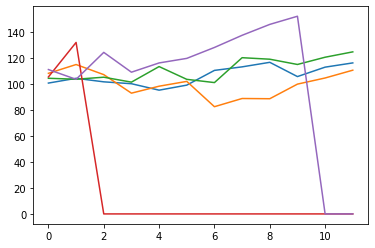
\includegraphics{images/barrier-example.png}
\end{figure}

\section{Simulated Paths for the Underlying Share and Counterparty Firm
}

 In order to simulate paths for the underlying share and the firm, a matrix of correlated prices is generated based on the requirement for a correlation of 0.2. 
 
    \begin{tcolorbox}[breakable, size=fbox, boxrule=1pt, pad at break*=1mm,colback=cellbackground, colframe=cellborder]
\prompt{In}{incolor}{4}{\boxspacing}
\begin{Verbatim}[commandchars=\\\{\}]
\PY{k}{def} \PY{n+nf}{share\PYZus{}path}\PY{p}{(}\PY{n}{S\PYZus{}0}\PY{p}{,} \PY{n}{risk\PYZus{}free\PYZus{}rate}\PY{p}{,} \PY{n}{sigma}\PY{p}{,} \PY{n}{Z}\PY{p}{,} \PY{n}{dT}\PY{p}{)}\PY{p}{:}
    \PY{k}{return} \PY{n}{S\PYZus{}0}\PY{o}{*}\PY{n}{np}\PY{o}{.}\PY{n}{exp}\PY{p}{(}\PY{n}{np}\PY{o}{.}\PY{n}{cumsum}\PY{p}{(}\PY{p}{(}\PY{n}{risk\PYZus{}free\PYZus{}rate}\PY{o}{\PYZhy{}}\PY{n}{sigma}\PY{o}{*}\PY{o}{*}\PY{l+m+mi}{2}\PY{o}{/}\PY{l+m+mi}{2}\PY{p}{)}\PY{o}{*}\PY{n}{dT} \PY{o}{+} \PY{n}{sigma}\PY{o}{*}\PY{n}{np}\PY{o}{.}\PY{n}{sqrt}\PY{p}{(}\PY{n}{dT}\PY{p}{)}\PY{o}{*}\PY{n}{Z}\PY{p}{,}\PY{l+m+mi}{1}\PY{p}{)}\PY{p}{)}


\PY{k}{def} \PY{n+nf}{generate\PYZus{}share\PYZus{}and\PYZus{}firm\PYZus{}price}\PY{p}{(}\PY{n}{S0}\PY{p}{,} \PY{n}{v\PYZus{}0}\PY{p}{,} \PY{n}{risk\PYZus{}free}\PY{p}{,} \PY{n}{sigma}\PY{p}{,} \PY{n}{sigma\PYZus{}firm}\PY{p}{,} \PY{n}{corr}\PY{p}{,} \PY{n}{T}\PY{p}{,} \PY{n}{sample\PYZus{}size} \PY{o}{=} \PY{l+m+mi}{10}\PY{p}{,} \PY{n}{timesteps} \PY{o}{=} \PY{l+m+mi}{12}\PY{p}{)}\PY{p}{:}
    \PY{n}{corr\PYZus{}matrix} \PY{o}{=} \PY{n}{np}\PY{o}{.}\PY{n}{array}\PY{p}{(}\PY{p}{[}\PY{p}{[}\PY{l+m+mi}{1}\PY{p}{,} \PY{n}{corr}\PY{p}{]}\PY{p}{,} \PY{p}{[}\PY{n}{corr}\PY{p}{,} \PY{l+m+mi}{1}\PY{p}{]}\PY{p}{]}\PY{p}{)}
    \PY{n}{norm\PYZus{}matrix} \PY{o}{=} \PY{n}{stats}\PY{o}{.}\PY{n}{norm}\PY{o}{.}\PY{n}{rvs}\PY{p}{(}\PY{n}{size} \PY{o}{=} \PY{n}{np}\PY{o}{.}\PY{n}{array}\PY{p}{(}\PY{p}{[}\PY{n}{sample\PYZus{}size}\PY{p}{,} \PY{l+m+mi}{2}\PY{p}{,} \PY{n}{timesteps}\PY{p}{]}\PY{p}{)}\PY{p}{)}
    \PY{n}{corr\PYZus{}norm\PYZus{}matrix} \PY{o}{=} \PY{n}{np}\PY{o}{.}\PY{n}{matmul}\PY{p}{(}\PY{n}{np}\PY{o}{.}\PY{n}{linalg}\PY{o}{.}\PY{n}{cholesky}\PY{p}{(}\PY{n}{corr\PYZus{}matrix}\PY{p}{)}\PY{p}{,} \PY{n}{norm\PYZus{}matrix}\PY{p}{)}
    
    \PY{n}{share\PYZus{}price\PYZus{}path} \PY{o}{=} \PY{n}{pd}\PY{o}{.}\PY{n}{DataFrame}\PY{p}{(}\PY{n}{share\PYZus{}path}\PY{p}{(}\PY{n}{S0}\PY{p}{,} \PY{n}{risk\PYZus{}free}\PY{p}{,} \PY{n}{sigma}\PY{p}{,} \PY{n}{Z}\PY{o}{=}\PY{n}{corr\PYZus{}norm\PYZus{}matrix}\PY{p}{[}\PY{p}{:}\PY{p}{,}\PY{l+m+mi}{0}\PY{p}{,}\PY{p}{]}\PY{p}{,} \PY{n}{dT}\PY{o}{=}\PY{l+m+mi}{1}\PY{o}{/}\PY{n}{timesteps}\PY{p}{)}\PY{p}{)}
    \PY{n}{share\PYZus{}price\PYZus{}path} \PY{o}{=} \PY{n}{share\PYZus{}price\PYZus{}path}\PY{o}{.}\PY{n}{transpose}\PY{p}{(}\PY{p}{)}

    \PY{n}{firm\PYZus{}price\PYZus{}path} \PY{o}{=} \PY{n}{pd}\PY{o}{.}\PY{n}{DataFrame}\PY{p}{(}\PY{n}{share\PYZus{}path}\PY{p}{(}\PY{n}{v\PYZus{}0}\PY{p}{,} \PY{n}{risk\PYZus{}free}\PY{p}{,} \PY{n}{sigma\PYZus{}firm}\PY{p}{,} \PY{n}{Z}\PY{o}{=}\PY{n}{corr\PYZus{}norm\PYZus{}matrix}\PY{p}{[}\PY{p}{:}\PY{p}{,}\PY{l+m+mi}{1}\PY{p}{,}\PY{p}{]}\PY{p}{,} \PY{n}{dT}\PY{o}{=}\PY{l+m+mi}{1}\PY{o}{/}\PY{n}{timesteps}\PY{p}{)}\PY{p}{)}
    \PY{n}{firm\PYZus{}price\PYZus{}path} \PY{o}{=} \PY{n}{firm\PYZus{}price\PYZus{}path}\PY{o}{.}\PY{n}{transpose}\PY{p}{(}\PY{p}{)}

    \PY{k}{return} \PY{p}{[}\PY{n}{share\PYZus{}price\PYZus{}path}\PY{p}{,}\PY{n}{firm\PYZus{}price\PYZus{}path}\PY{p}{]}  
\end{Verbatim}
\end{tcolorbox}

A Pearson test can be used to verify that the correlation is very close to the 0.2 target value. In Python this can be achieved as follows.

    \begin{tcolorbox}[breakable, size=fbox, boxrule=1pt, pad at break*=1mm,colback=cellbackground, colframe=cellborder]
\prompt{In}{incolor}{5}{\boxspacing}
\begin{Verbatim}[commandchars=\\\{\}]
\PY{c+c1}{\PYZsh{}Testing share and firm price correlation}
\PY{n}{sample\PYZus{}size} \PY{o}{=} \PY{l+m+mi}{20}
\PY{n}{test} \PY{o}{=} \PY{n}{generate\PYZus{}share\PYZus{}and\PYZus{}firm\PYZus{}price}\PY{p}{(}\PY{n}{S0}\PY{p}{,} \PY{n}{v\PYZus{}0}\PY{p}{,} \PY{n}{risk\PYZus{}free}\PY{p}{,} \PY{n}{sigma}\PY{p}{,} \PY{n}{sigma\PYZus{}firm}\PY{p}{,} \PY{n}{corr}\PY{p}{,} \PY{n}{T}\PY{p}{,} \PY{n}{sample\PYZus{}size}\PY{p}{,} \PY{n}{timesteps} \PY{o}{=} \PY{l+m+mi}{20000}\PY{p}{)}

\PY{n}{share\PYZus{}ret} \PY{o}{=} \PY{n}{np}\PY{o}{.}\PY{n}{log}\PY{p}{(}\PY{n}{test}\PY{p}{[}\PY{l+m+mi}{0}\PY{p}{]}\PY{p}{)}

\PY{k}{for} \PY{n}{i} \PY{o+ow}{in} \PY{n+nb}{range}\PY{p}{(}\PY{n}{sample\PYZus{}size}\PY{p}{)}\PY{p}{:}
    \PY{n}{test}\PY{p}{[}\PY{l+m+mi}{0}\PY{p}{]}\PY{p}{[}\PY{l+s+s1}{\PYZsq{}}\PY{l+s+s1}{sharelog}\PY{l+s+s1}{\PYZsq{}}\PY{p}{]} \PY{o}{=} \PY{n}{np}\PY{o}{.}\PY{n}{log}\PY{p}{(}\PY{n}{test}\PY{p}{[}\PY{l+m+mi}{0}\PY{p}{]}\PY{p}{[}\PY{n}{i}\PY{p}{]}\PY{p}{)}
    \PY{n}{test}\PY{p}{[}\PY{l+m+mi}{1}\PY{p}{]}\PY{p}{[}\PY{l+s+s1}{\PYZsq{}}\PY{l+s+s1}{firmlog}\PY{l+s+s1}{\PYZsq{}}\PY{p}{]} \PY{o}{=} \PY{n}{np}\PY{o}{.}\PY{n}{log}\PY{p}{(}\PY{n}{test}\PY{p}{[}\PY{l+m+mi}{1}\PY{p}{]}\PY{p}{[}\PY{n}{i}\PY{p}{]}\PY{p}{)}
    \PY{n+nb}{print}\PY{p}{(}\PY{n}{stats}\PY{o}{.}\PY{n}{pearsonr}\PY{p}{(}\PY{n}{test}\PY{p}{[}\PY{l+m+mi}{0}\PY{p}{]}\PY{p}{[}\PY{l+s+s1}{\PYZsq{}}\PY{l+s+s1}{sharelog}\PY{l+s+s1}{\PYZsq{}}\PY{p}{]}\PY{o}{.}\PY{n}{diff}\PY{p}{(}\PY{p}{)}\PY{o}{.}\PY{n}{dropna}\PY{p}{(}\PY{p}{)}\PY{p}{,} \PY{n}{test}\PY{p}{[}\PY{l+m+mi}{1}\PY{p}{]}\PY{p}{[}\PY{l+s+s1}{\PYZsq{}}\PY{l+s+s1}{firmlog}\PY{l+s+s1}{\PYZsq{}}\PY{p}{]}\PY{o}{.}\PY{n}{diff}\PY{p}{(}\PY{p}{)}\PY{o}{.}\PY{n}{dropna}\PY{p}{(}\PY{p}{)}\PY{p}{)}\PY{p}{)}
\end{Verbatim}
\end{tcolorbox}

    \begin{Verbatim}[commandchars=\\\{\}]
(0.2035028479587627, 6.07336614624919e-186)
(0.1986599648970965, 4.04999708397334e-177)
(0.2016759847597355, 1.3775160789695309e-182)
(0.20364055709605317, 3.381815103189066e-186)
(0.19385401550478024, 1.3726860317349184e-168)
(0.19892212605701942, 1.3666646645127986e-177)
(0.18344242259502544, 7.064732561303709e-151)
(0.20519864966486748, 4.356484560250648e-189)
(0.193927020114363, 1.022531700201078e-168)
(0.19751037260327703, 4.659785935918803e-175)
(0.20393895669991588, 9.495454795149592e-187)
(0.20458792743312265, 5.953557128978809e-188)
(0.2042028358117276, 3.0829601588859696e-187)
(0.19512700379639908, 7.943982338391081e-171)
(0.19603082201925184, 2.003660281095667e-172)
(0.19820752618175266, 2.630853001655849e-176)
(0.20299979761482267, 5.137198920374959e-185)
(0.1966663418793928, 1.4903037901828931e-173)
(0.20319824398313788, 2.214204369119104e-185)
(0.20765530182748704, 1.0810080941108714e-193)
    \end{Verbatim}

The payoff calculation for the up-and-out barrier option is defined as follows.

    \begin{tcolorbox}[breakable, size=fbox, boxrule=1pt, pad at break*=1mm,colback=cellbackground, colframe=cellborder]
\prompt{In}{incolor}{11}{\boxspacing}
\begin{Verbatim}[commandchars=\\\{\}]
\PY{c+c1}{\PYZsh{} define payoff for up\PYZhy{}and\PYZhy{}out call option}
\PY{k}{def} \PY{n+nf}{payoff}\PY{p}{(}\PY{n}{S\PYZus{}t}\PY{p}{,} \PY{n}{K}\PY{p}{,} \PY{n}{L}\PY{p}{)}\PY{p}{:}
    \PY{n}{stopped\PYZus{}S} \PY{o}{=} \PY{n}{S\PYZus{}t}\PY{o}{.}\PY{n}{iloc}\PY{p}{[}\PY{o}{\PYZhy{}}\PY{l+m+mi}{1}\PY{p}{]}\PY{o}{.}\PY{n}{where}\PY{p}{(}\PY{p}{(}\PY{n}{S\PYZus{}t} \PY{o}{\PYZlt{}} \PY{n}{L}\PY{p}{)}\PY{o}{.}\PY{n}{all}\PY{p}{(}\PY{p}{)}\PY{p}{,} \PY{l+m+mi}{0}\PY{p}{)}
    \PY{k}{return} \PY{n}{np}\PY{o}{.}\PY{n}{maximum}\PY{p}{(}\PY{n}{stopped\PYZus{}S} \PY{o}{\PYZhy{}} \PY{n}{K}\PY{p}{,} \PY{l+m+mi}{0}\PY{p}{)}\PY{o}{.}\PY{n}{to\PYZus{}numpy}\PY{p}{(}\PY{p}{)}

\PY{n}{payoff}\PY{p}{(}\PY{n}{share\PYZus{}price\PYZus{}12\PYZus{}months}\PY{p}{,} \PY{n}{K}\PY{p}{,} \PY{n}{L}\PY{p}{)}
\end{Verbatim}
\end{tcolorbox}

The simulated payoff paths over twelve months are plotted below, with an arbitrary starting value of 200 for the firm value.

\begin{figure}
    \centering
    \caption{Simulated Payoff Paths over 12 Months}
    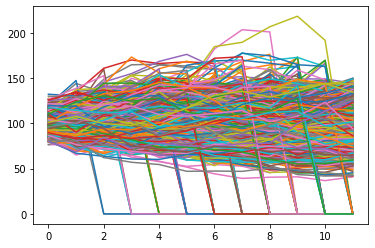
\includegraphics{images/all-paths.png}
\end{figure}

\section{Monte Carlo Estimations
}

\subsection{Default-Free Value Estimation}
\begin{figure}
    \centering
    \caption{Simulated Payoff Paths over 12 Months}
    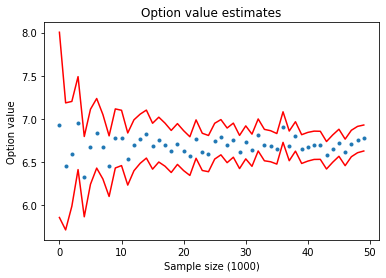
\includegraphics{images/default-free.png}
\end{figure}

\subsection{Credit Valuation Adjustment Estimation}



\section{Monte Carlo estimates for the price of the option incorporating counterparty risk, given by the default-free price less the CVA.}

    \begin{tcolorbox}[breakable, size=fbox, boxrule=1pt, pad at break*=1mm,colback=cellbackground, colframe=cellborder]
\prompt{In}{incolor}{1}{\boxspacing}
\begin{Verbatim}[commandchars=\\\{\}]
\PY{k+kn}{import} \PY{n+nn}{QuantLib} \PY{k}{as} \PY{n+nn}{ql}
\PY{k+kn}{from} \PY{n+nn}{collections} \PY{k+kn}{import} \PY{n}{namedtuple}
\PY{k+kn}{import} \PY{n+nn}{math}
\end{Verbatim}
\end{tcolorbox}

    \begin{tcolorbox}[breakable, size=fbox, boxrule=1pt, pad at break*=1mm,colback=cellbackground, colframe=cellborder]
\prompt{In}{incolor}{2}{\boxspacing}
\begin{Verbatim}[commandchars=\\\{\}]
\PY{n}{today} \PY{o}{=} \PY{n}{ql}\PY{o}{.}\PY{n}{Date}\PY{p}{(}\PY{l+m+mi}{15}\PY{p}{,} \PY{n}{ql}\PY{o}{.}\PY{n}{February}\PY{p}{,} \PY{l+m+mi}{2020}\PY{p}{)}\PY{p}{;}
\PY{n}{settlement}\PY{o}{=} \PY{n}{ql}\PY{o}{.}\PY{n}{Date}\PY{p}{(}\PY{l+m+mi}{19}\PY{p}{,} \PY{n}{ql}\PY{o}{.}\PY{n}{February}\PY{p}{,} \PY{l+m+mi}{2020}\PY{p}{)}\PY{p}{;}
\PY{n}{ql}\PY{o}{.}\PY{n}{Settings}\PY{o}{.}\PY{n}{instance}\PY{p}{(}\PY{p}{)}\PY{o}{.}\PY{n}{evaluationDate} \PY{o}{=} \PY{n}{today}\PY{p}{;}
\PY{n}{term\PYZus{}structure} \PY{o}{=} \PY{n}{ql}\PY{o}{.}\PY{n}{YieldTermStructureHandle}\PY{p}{(}
    \PY{n}{ql}\PY{o}{.}\PY{n}{FlatForward}\PY{p}{(}\PY{n}{settlement}\PY{p}{,}\PY{l+m+mf}{0.04875825}\PY{p}{,}\PY{n}{ql}\PY{o}{.}\PY{n}{Actual365Fixed}\PY{p}{(}\PY{p}{)}\PY{p}{)}
    \PY{p}{)}
\PY{n}{index} \PY{o}{=} \PY{n}{ql}\PY{o}{.}\PY{n}{Euribor1Y}\PY{p}{(}\PY{n}{term\PYZus{}structure}\PY{p}{)}
\end{Verbatim}
\end{tcolorbox}



    \begin{Verbatim}[commandchars=\\\{\}]
--------------------------------------------------------------------------------
--
    Model Price    Market Price     Implied Vol      Market Vol       Rel Error
--------------------------------------------------------------------------------
--
        0.00871         0.00949         0.10531         0.11480        -0.08263
        0.00968         0.01008         0.10634         0.11080        -0.04018
        0.00867         0.00871         0.10652         0.10700        -0.00448
        0.00653         0.00625         0.10665         0.10210         0.04442
        0.00357         0.00334         0.10680         0.10000         0.06773
--------------------------------------------------------------------------------
--
Cumulative Error :         0.12288
    \end{Verbatim}

\section{Conclusion}



\newpage
\section*{} \label{bibsection}


% the second parameter MMMMM should be as long as the longest label you use, in my case Smoller -- if you use % numbers only, use 99
% use \cite{refname} to refer to bibliography item \bibitem{refname} 
% LaTeX assigns a number, unless you use \bibitem[Name]{refname} -- in this case
% LaTeX prints Name when you use \cite{refname}
\begin{thebibliography}{MMMMM} 
\bibitem{BA1} Blanchard, Arnaud. "The two-factor Hull-White model: pricing and calibration of interest rates derivatives." KTH Royal Insitute of Technology (2014).


\end{thebibliography}
\bibliographystyle{plain}
\bibliography{template}

\end{document}
